\section{Tareas de usuario}
\label{sec::usertasks}

Por \'ultimo describiremos las tareas de usuario programas para demostrar el
uso de las facilidades de Sistema Operativo que hemos implementado. En primera instancia
describiremos el formato ELF usado para las tareas y luego describiremos las tareas mismas
que hemos programado.

\subsection{Formato ELF}

Para facilitar la implementaci\'on de las tareas, se decidi\'o utilizar C como lenguaje de
implementaci\'on. Tambi\'en era nuestro inter\'es poder disponer de una librer\'ia separable
de funciones y wrappers del c\'odigo espec\'fico para el Sistema Operativo, de manera de poder
tener una separaci\'on de m\'odulos y as\'i favorecer la simplicidad de desarrollo de las tareas.
Por ejemplo, nos pareci\'o importante poder mantener una secci\'on de datos (\texttt{.data}),
secciones reservadas de espacio de memoria (\texttt{.bss}) y secciones de constantes (\texttt{.rodata})
de manera de poder emplear buffers est\'aticos de memoria (para superar temporalmente la limitaci\'on de
falta de memoria de \textit{heap} en las tareas).

Ambos objetivos hicieron entonces que fuera necesario que el Sistema Operativo pudiese, como
m\'inimo, soportar la carga de ELFs est\'aticos. Esto era una soluci\'on a todos los problemas
planteados anteriormente: es muy sencillo compilar c\'odigo en C a archivo objeto y linkear todos
estos en un ejecutable ELF est\'atico final, mediante el uso de un compilador como GCC y un linker como
LD.

Para ello primero describiremos el formato ELF est\'atico ejecutable. El mismo es muy sencillo y consiste
de las siguientes partes:

\begin{itemize}
	\item Un \textit{header} identificador con constantes para comprender y parsear el resto del archivo. Los que
	resultaron importantes para nuestros prop\'ositos son los siguientes:

		\begin{itemize}
			\item 16 bytes m\'agicos: el valor 0x7F y los caracteres ASCII E, L y F y otros valores m\'agicos
			que permiten identificar y diferenciar el header de este tipo de ejecutables. En particular dos de estos
			n\'umeros m\'agicos que nos interesan son el 4 (contando desde 0), que corresponde a si es un binario de 32 bits,
			y el 5 que corresponde a si el binario tiene sus valores multibyte encondeados mediante Little Endian y usando
			complemento a dos.
			\item El tipo de binario ELF: En este caso nos interesa el tipo 2: Executable Files.
			\item La version del binario ELF. No nos interesa en particular este valor.
			\item Punto de entrada: Direcci\'on de memoria virtual donde inicia el c\'odigo de este ejecutable (puesto que
			estamos considerando solamente el caso de binario ELF ejecutable).
			\item Offset al comienzo de la tabla de headers de programa. Estos son los segmentos de memoria que necesitamos
			crear y copiar en memoria virtual para poder tener la im\'agen de este proceso corriendo.
			\item Contador de cantidad de secciones de program headers.
			\item Tama\~no de una secci\'on de program header (para poder cargarlo e interpretarlo).
		\end{itemize}
	
	Los dem\'as valores de este header no son utilizados, ya que corresponden a por ejemplo la tabla de secciones y s\'imbolos para
	un archivo objeto linkeable y dem\'as valores.

	\item Un header de programa para cada secci\'on relevante. Cada uno de estos consiste de:

	\begin{itemize}
		\item Un flag de tipo. En nuestro caso particular solo nos interesan los que son del tipo ELF\_LOAD, valor $0x1$, correspondiente
		a un segmento cargable. En particular esto implica que el kernel no soporta cargar binarios linkeados din\'amicamente. Esto es una
		limitaci\'on aunque si le interesa al lector hay una discusi\'on sobre si realmente linkear din\'amicamente con librer\'ias tiene
		beneficios~\footnote{\url{http://harmful.cat-v.org/software/dynamic-linking/}}.	
		\item Un offset al inicio de esta secci\'on en la im\'agen de archivo cargada a memoria. De ahi obtenemos los datos correspondientes
		a este segmento.
		\item La direcci\'on virtual donde debemos cargar este m\'odulo. 
		\item La direcci\'on f\'isica donde debemos cargar este m\'odulo si es pertinente. Dado que el entorno de desarrollo empleado es GNU
		Toolchain en Linux, este valor no es relevante a nuestros prop\'ositos.
		\item Tama\~no en archivo en bytes de la secci\'on.
		\item Tama\~no en memoria en bytes de la secci\'on. Estos dos valores pueden diferir ya que una secci\'on puede consistir en una
		indicaci\'on al sistema de que debe reservar una cantidad determinada de memoria. Un ejemplo de este tipo de secciones son las
		secciones \texttt{.bss} que surgen de reservar arreglos est\'aticos en por ejemplo un programa en C.
		\item Flags. Estos flags indican por ejemplo si la secci\'on es una secci\'on ejecutable, de lectura y de escritura. Se usa por
		ejemplo para reservar p\'aginas con permisos acordes.
		\item Requerimientos de alineaci\'on. Generalmente se requiere que los datos esten alineados a p\'aginas de 4 KB.
	\end{itemize}
\end{itemize}

	Con estos datos podemos entonces parsear el archivo elf y generar el mapeo de p\'aginas acorde de manera muy sencilla, que es exactamente
	lo que realizan los algoritmos. En particular \texttt{elf\_overlay\_image} toma un archivo ELF v\'alido (seg\'un nuestras precondiciones)
	y crea el mapa de p\'aginas acorde en el directorio de p\'aginas actual. Esto se usa para inicializar la tarea \texttt{init} y luego se
	usa en la llamada a sistema \texttt{exec}.
	
	Un esquema de un ejecutable ELF se encuentra en
	la Figura~\ref{fig::elf}.

	\begin{figure}[H]
		\caption{Diagrama de un ejecutable ELF, mostrando la estructura a alto nivel. Tomado de http://tldp.org/LDP/tlk/kernel/elf.gif} 
		\label{fig::elf}
		\centering
		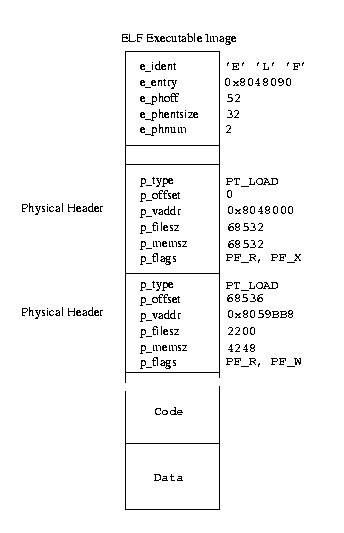
\includegraphics[width=0.4\textwidth]{elf.png}
	\end{figure}

	M\'as detalles sobre el formato ELF se pueden encontrar en ~\cite{abi}.

\subsection{Consola}

La principal tarea de usuario que implementamos es la consola
o Shell. Esta se ocupa de interpretar comandos (tomados por teclado) y responder
a los mismos de manera acorde.

Es la consola quien en primera instancia abre el terminal para lectura y para escritura
(los procesos luego heredan los descriptores de archivos asignados). El interprete de
comandos acepta una gram\'atica de la forma:

\begin{verbatim}
	comando := "" | programa lista_argumentos "\n"
	lista_argumentos := "\n" | [caracteres] (' ' | '\t')
\end{verbatim}

es decir, una lista de un comando y argumentos correspondientes a lo que uno esperar\'ia
viniendo de un terminal de consola como los de Unix o DOS.

El Shell parsea entonces comandos como l\'ineas y luego realiza el siguiente proceso:

\begin{itemize}
	\item Si el comando corresponde a una funci\'on de consola (por ejemplo el comando \texttt{cd}
	para cambiar de directorio), se ejecuta una funci\'on manejadora de este comando.
	\item Si no es as\'i, La consola forkea un proceso hijo.
	\item El subproceso recien creado realiza exec para	``convertirse'' en el comando que queremos ejecutar. 
	Los argumentos son pusheados a la pila de este proceso mientras se realiza la llamada a sistema \texttt{exec}, 
	de manera que al ejecutarse la tarea dispone de los mismos mediante \texttt{argc} y \texttt{argv} como uno 
	esperar\'ia que ocurre en la mayor\'ia de los Sistemas Operativos basados en UNIX o en DOS.
	\item La consola espera a que termine este proceso hijo de ejecutarse.
	\item El proceso hijo realiza su trabajo y luego ejecuta la llamada a sistema \texttt{exit} para liberar
	el procesador.
	\item La consola retoma entonces el control.
\end{itemize}

Como podemos ver la implementaci\'on sigue los lineamientos que uno esperar\'ia de una consola de sistema muy b\'asica,
como esta explicado en~\cite{systemv}.

\subsection{Tareas implementadas}

Para demostrar un subconjunto de funcionalidad, implementamos las siguientes tareas y comandos espec\'ificos de consola

\begin{itemize}
	\item echo, devuelve por consola todos los par\'ametros que le son dados.
	\item date, devuelve por consola la fecha y hora
	\item ls, devuelve el contenido del directorio indicado si es llamado con argumentos y
	el del directorio actual si no se le pasan argumentos.
	\item cat, devuelve por consola el contenido del archivo pasado por par\'ametro.
	\item cp, copia (creandolo si es necesario) un archivo con nombre pasado por par\'ametro a otro lugar 
	pasado tambi\'en por par\'ametro.
\end{itemize}
